\documentclass[10pt,dvipsnames]{beamer}

%\usepackage{pgfpages}
%\mode<handout>{\setbeamercolor{background canvas}{bg=black!20}}
%\pgfpagesuselayout{4 on 1}[letterpaper,border shrink=5mm]

\usepackage{lmodern}
\usepackage{xcolor}
\usepackage[utf8]{inputenc}
\usepackage{amsmath, amsfonts}
\usepackage{verbatim}
\usepackage{fancyvrb}
\usepackage{tikz}
\usetikzlibrary{decorations.pathreplacing}
\beamertemplatenavigationsymbolsempty
\setbeamertemplate{footline}[frame number]
\addtolength{\oddsidemargin}{-3pt}

\definecolor{dgreen}{rgb}{0.,0.6,0.}
\definecolor{highlight}{rgb}{0.,0.6,0.}

\definecolor{my_example_color}{rgb}{0.1,0.6,0.4}

\usepackage{multimedia}

\title{Cancer classification based on miRNA profiles using ASP} 
\author{K. Becker and H. Klarner}
\date{Berlin, Mai 2016}
\institute{
Freie Universität Berlin, Germany
}
% logo of my university
\titlegraphic{\vfill
\includegraphics[width=2cm]{FU-Logo}\hspace*{4.75cm}~%
   
\includegraphics[width=2cm]{BMBF-Logo}
}

\begin{document}


\frame{\titlepage}


%{\tiny R. Thomas. "Regulatory networks seen as asynchronous automata." JTB, 1991}


\begin{frame}{Selective cell targeting}
\large
\begin{itemize}
\item \textbf{Problem:} Discrimination of tumor from healthy tissues
\end{itemize}
\vspace{0.5cm}
\begin{center}
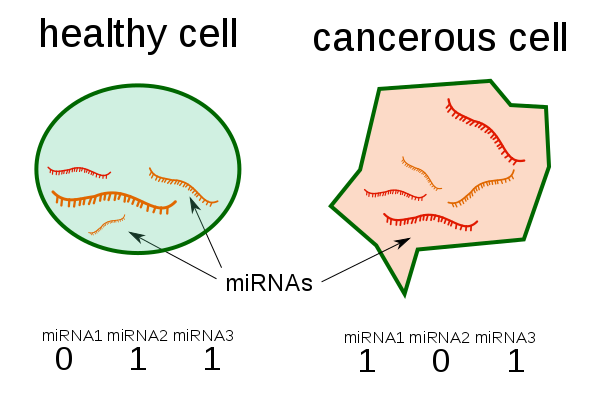
\includegraphics[scale=0.3]{cells1.png}
\end{center}
\vspace{0.5cm}
\begin{itemize}
\item \textbf{Idea:} Cells differ in miRNA profiles\\
$\rightarrow$ \textbf{in vitro classification using biochemical circuits}
\end{itemize}
\end{frame}


\begin{frame}{A boolean expression in conjunctive normal form (CNF)}
\begin{itemize}
\item conjunction (AND) of \emph{gates}
\item each gate is a disjunction (OR) of literals
\item \textbf{example:}  
\begin{align*}
(a + b + !c) * (d + e) * (!f)
\end{align*}
{\small $+$ means disjunction, $*$ means conjunction, $!$ means negation}
\vspace{0.2cm}
\item CNF evaluates to 1 (\emph{predicts cancer}) iff every gate evaluates to 1
\end{itemize}
\vspace{0.2cm}
\begin{center}
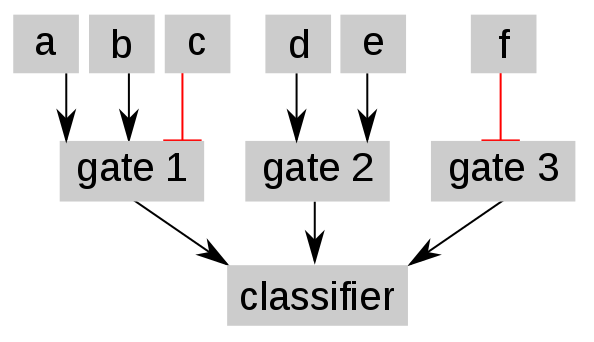
\includegraphics[scale=0.25]{classifier_exp.png}
\end{center}
\end{frame}


\begin{frame}{Constraints from biology}
\begin{itemize}
 \item less than 10 inputs in total
 \item no more than 6 inputs attached to the AND gate
 \item no more than 3 inputs atttached to any OR gate
 \item no NOT gates attached to an OR gate
 \item no more than 2 OR gates
 \item no more than 4 NOT gates
\end{itemize}
\begin{center}
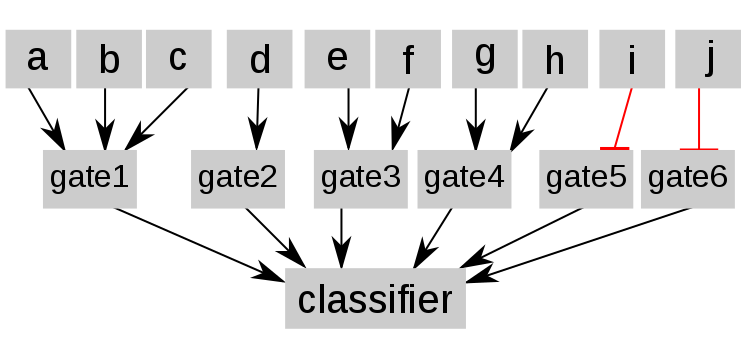
\includegraphics[scale=0.3]{classifier_max.png}
\end{center}
\end{frame}


\begin{frame}{Our encoding in ASP - Reminder}
  \begin{itemize}
  \item facts:
 \end{itemize}
 \begin{center}
  \texttt{ P(A). }
 \end{center}
 
 \vspace{0.5cm} 
   \begin{itemize}
  \item conditional constraints:
 \end{itemize}
 \begin{center}
  \texttt{ Q(A) :- P(A). }
 \end{center}

  \vspace{0.5cm} 
  \begin{itemize}
  \item count constraints:
 \end{itemize}
 \begin{center}
  \texttt{ X \{ Q(A,B) \} Y. }
 \end{center}

 \vspace{0.5cm} 
 \begin{itemize}
  \item conditional count constraints:
 \end{itemize}
 \begin{center}
  \texttt{ X \{ Q(A,B) \} Y :- P(A). }
 \end{center}

  \vspace{0.5cm} 
  \begin{itemize}
  \item integrity constraints:
 \end{itemize}
  \begin{center}
  \texttt{ :- P(A). }
 \end{center}
\end{frame}


\begin{frame}[fragile]{Input: Data}
\begin{center}
\begin{tabular}{|c|c|c|c|c|}
\hline
ID&	Annots&	g1&	g2&	g3\\
\hline
1&	0&	1&	1&	0\\
2&	0&	0&	0&	1\\
3&	1&	0&	1&	0\\
\hline
\end{tabular}
\begin{tikzpicture}[overlay]
\draw[decorate, decoration={brace}]
      (-2.2,1.2) -- node[above=0.15cm, scale=1] {\textbf{miRNAs}} (-0.2,1.2);
\draw[decorate, decoration={brace}]
      (-3.8,1.2) -- node[above=0.15cm, scale=1] {\textbf{cancer?}} (-2.5,1.2);
\draw[decorate, decoration={brace}]
      (-5,-0.7) -- node[left=0.15cm, scale=1] {\textbf{tissues}} (-5,0.5);
\end{tikzpicture}
\end{center}
\vspace{0.2cm}
\color{my_example_color}
\begin{verbatim}
tissue(1,healthy). tissue(2,healthy). tissue(3,cancer).
 
data(1,g1,high). data(1,g2,high). data(1,g3,low).
data(2,g1,low).  data(2,g2,low).  data(2,g3,high).
data(3,g1,low).  data(3,g2,high). data(3,g3,low).
 
is_mirna(Y) :- data(X,Y,Z).
\end{verbatim}
\end{frame}



\begin{frame}[fragile]{Input: Classifier structure}
\begin{center}
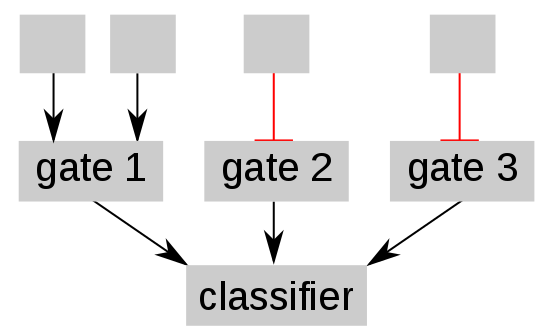
\includegraphics[scale=0.18]{classifier.png}
\end{center}
\color{my_example_color}\small
\begin{verbatim}
is_gate_type(1..2).

upper_bound_pos_inputs(type1, 2).
upper_bound_neg_inputs(type1, 0).
lower_bound_pos_inputs(type1, 0).
lower_bound_neg_inputs(type1, 0).
upper_bound_gate_occurence(type1, 1).

upper_bound_pos_inputs(type2, 0).
upper_bound_neg_inputs(type2, 1).
lower_bound_pos_inputs(type2, 0).
lower_bound_neg_inputs(type2, 0).
upper_bound_gate_occurence(type2, 2).

upper_bound_total_inputs(4).
\end{verbatim}
\end{frame}


\begin{frame}[fragile]{Decision 1: How many gates do we use?}

\small
\begin{minipage}{0.45\textwidth}
\color{my_example_color}
\begin{verbatim}
number_of_gates(2).

is_gate_id(1).
is_gate_id(2).
\end{verbatim}

\end{minipage}
\hfill
\begin{minipage}{0.45\textwidth}
\begin{center}
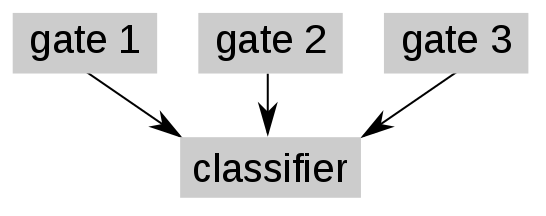
\includegraphics[scale=0.3]{exp1.png}
\end{center}
\end{minipage}
\vspace{1.3cm}

\begin{verbatim}
1 {number_of_gates(1..3)} 1.

is_integer(1..3).
is_gate_id(GateID) :- number_of_gates(X),is_integer(GateID), 
                      GateID<=X.
\end{verbatim}
\end{frame}


\begin{frame}[fragile]{Decision 2: What is the gate type of each gate?}
\small
\begin{minipage}{0.45\textwidth}
\color{my_example_color}
\begin{verbatim}
gate_type(1, type1).
gate_type(2, type2).
\end{verbatim}
\end{minipage}
\hfill
\begin{minipage}{0.45\textwidth}
\begin{center}
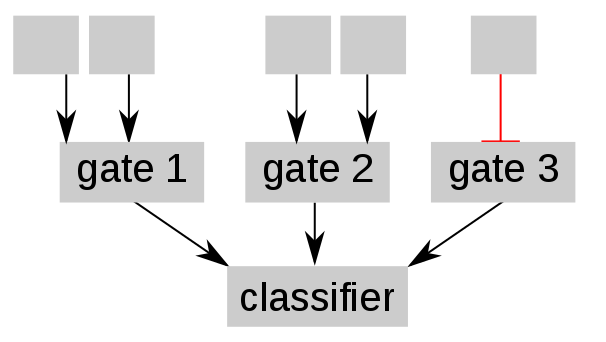
\includegraphics[scale=0.3]{exp2.png}
\end{center}
\end{minipage}
\vspace{1.3cm}
\begin{verbatim}
1 {gate_type(GateID, X) : is_gate_type(X)} 1 :- is_gate_id(GateID).
\end{verbatim}
\end{frame}


\begin{frame}[fragile]{Decision 3: What are the inputs for our gates?}
\vspace{0.3cm}
\small
\begin{minipage}{0.45\textwidth}
\color{my_example_color}
\begin{verbatim}
gate_input(1,positive,g2).
gate_input(2,negative,g1).
\end{verbatim}
\end{minipage}
\hfill
\begin{minipage}{0.45\textwidth}
\begin{center}
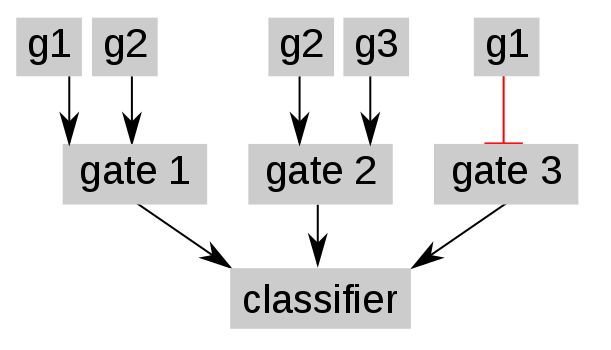
\includegraphics[scale=0.2]{exp3.png}
\end{center}
\end{minipage}
\vspace{0.5cm}

\begin{Verbatim}
X {gate_input(GateID,positive,MiRNA):is_mirna(MiRNA)} Y 
   :-gate_type(GateID,GateType),
     lower_bound_pos_inputs(GateType,X), 
     upper_bound_pos_inputs(GateType,Y).

X {gate_input(GateID,negative,MiRNA):is_mirna(MiRNA)} Y 
   :-gate_type(GateID,GateType),
     lower_bound_neg_inputs(GateType,X),
     upper_bound_neg_inputs(GateType,Y).
\end{Verbatim}
\end{frame}




\begin{frame}[fragile]{Safety: Gates must have inputs}
 \begin{columns}  
 \begin{column}{0.5\textwidth}
 \begin{center}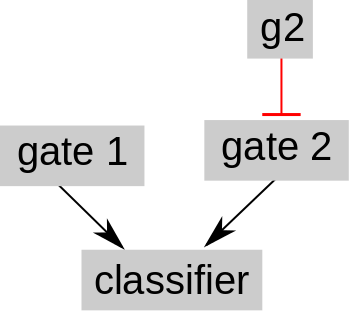
\includegraphics[width=3cm]{constraints_01.png}\end{center}
 \color{my_example_color}
 \begin{Verbatim}[fontsize=\small]
  is_gate_id(1).
  is_gate_id(2).
  gate_input(2,negative,g1).
 \end{Verbatim}
 \end{column}
 \begin{column}{0.5\textwidth}
 \begin{center}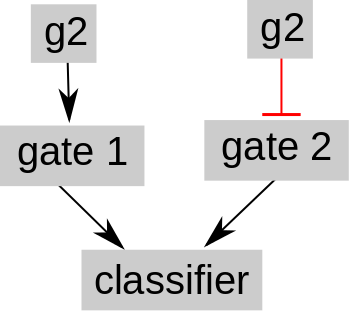
\includegraphics[width=3cm]{constraints_02.png}\end{center}
 \color{my_example_color}
 \begin{Verbatim}[fontsize=\small]
  is_gate_id(1).
  is_gate_id(2).
  gate_input(2,negative,g2).
  gate_input(2,negative,g2).
 \end{Verbatim}
 \end{column}
 \end{columns}
 \vspace{1cm}
 \texttt{
 1 \{gate\_input(GateID, Sign, MiRNA):\\
  \quad {\color{gray} is\_sign(Sign), is\_mirna(MiRNA)}\} :- is\_gate\_id(GateID).
 }
 
\end{frame}

\begin{frame}[fragile]{Inputs must be unique}
 \begin{columns}  
 \begin{column}{0.5\textwidth}
 \begin{center}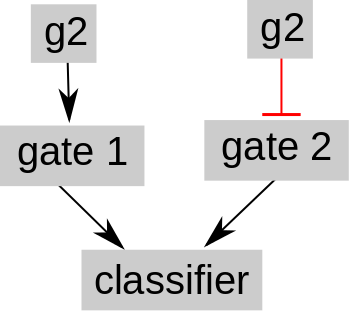
\includegraphics[width=3cm]{constraints_02.png}\end{center}
 \color{my_example_color}
  \begin{Verbatim}[fontsize=\small]
  is_mirna(g1). is_mirna(g2).
  is_mirna(g3).
  gate_input(1,positive,g2).
  gate_input(2,negative,g2).
 \end{Verbatim}
 \end{column}
 \begin{column}{0.5\textwidth}
 \begin{center}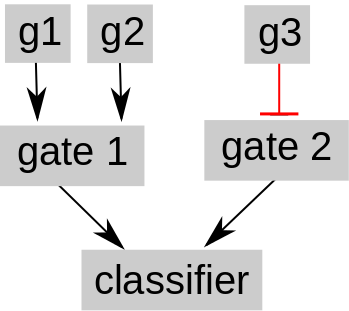
\includegraphics[width=3cm]{constraints_03.png}\end{center}
  \color{my_example_color}
  \begin{Verbatim}[fontsize=\small]
  is_mirna(g1). is_mirna(g2).
  is_mirna(g3).
  gate_input(1,positive,g1).
  gate_input(2,positive,g2).
  gate_input(2,negative,g3).
 \end{Verbatim}
 \end{column}
 \end{columns}
 \vspace{1cm}
 \texttt{
  \{gate\_input(GateID,Sign,MiRNA):\\
   \quad {\color{gray} is\_sign(Sign), is\_gate(GateID)}\} 1 :- is\_mirna(MiRNA).
 }
 
\end{frame}


\begin{frame}[fragile]{Number of inputs is bounded}
 \begin{columns}  
 \begin{column}{0.5\textwidth}
 \begin{center}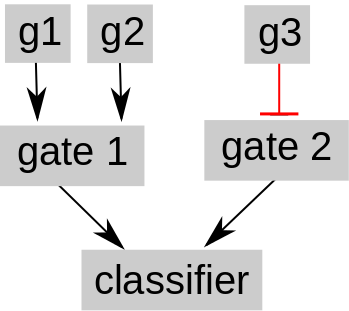
\includegraphics[width=3cm]{constraints_04.png}\end{center}
 \color{my_example_color}
  \begin{Verbatim}[fontsize=\small]
  upper_bound_inputs(2).
  gate_type(1,type1).
  gate_type(2,type2).
  gate_input(1,positive,g1).
  gate_input(2,positive,g2).
  gate_input(2,negative,g3).
 \end{Verbatim}
 \end{column}
 \begin{column}{0.5\textwidth}
 \begin{center}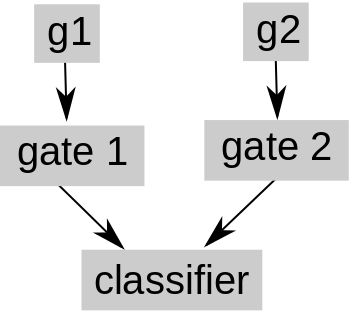
\includegraphics[width=3cm]{constraints_05.png}\end{center}
 \color{my_example_color}
  \begin{Verbatim}[fontsize=\small]
  upper_bound_inputs(2).
  gate_type(1,type1).
  gate_type(2,type1).
  gate_input(1,positive,g1).
  gate_input(2,positive,g2).
 \end{Verbatim}
 \end{column}
 \end{columns}
 \vspace{1cm}
 \texttt{
  \{gate\_input(GateID,Sign,MiRNA):\\
   \quad {\color{gray} is\_gate\_id(GateID), is\_sign(Sign), is\_mirna(MiRNA)}\} X :-\\
   \quad upper\_bound\_inputs(X).
 }
\end{frame}

\begin{frame}[fragile]{Occurences of gates}
 \begin{columns}  
 \begin{column}{0.6\textwidth}
 \begin{center}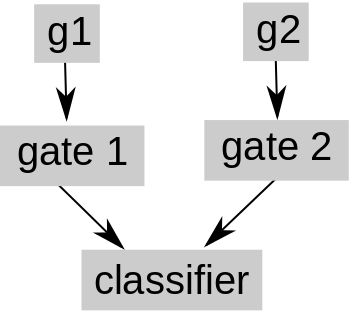
\includegraphics[width=3cm]{constraints_05.png}\end{center}
 \color{my_example_color}
  \begin{Verbatim}[fontsize=\small]
  upper_bound_gate_occurence(type1, 1).
  upper_bound_inputs(2).
  gate_type(1,type1).
  gate_type(2,type1).
  gate_input(1,positive,g1).
  gate_input(2,positive,g2).
 \end{Verbatim}
 \end{column}
 \begin{column}{0.6\textwidth}
 \begin{center}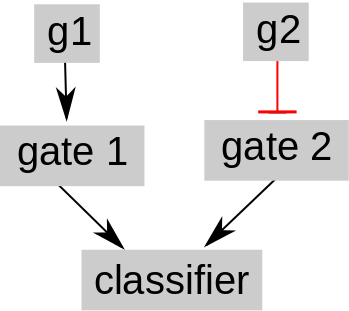
\includegraphics[width=3cm]{constraints_06.png}\end{center}
 \color{my_example_color}
  \begin{Verbatim}[fontsize=\small]
  upper_bound_gate_occurence(type1, 1).
  upper_bound_inputs(2).
  gate_type(1,type1).
  gate_type(2,type2).
  gate_input(1,positive,g1).
  gate_input(2,negative,g2).
 \end{Verbatim}
 \end{column}
 \end{columns}
 \vspace{1cm}
 \texttt{
  \{gate\_type(GateID,GateType):{\color{gray}\;is\_gate\_id(GateID)}\} X :-\\
     \quad upper\_bound\_gate\_occurence(GateType,X).
 }
\end{frame}
 

\begin{frame}[fragile]{Consistency of gates with data}
 \begin{columns}  
 \begin{column}{0.3\textwidth}
 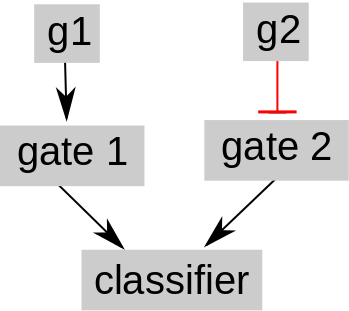
\includegraphics[width=3cm]{constraints_06.png}
 \end{column}
 \begin{column}{0.6\textwidth}
 \begin{tabular}{|c|c|c|c|c|c|c|}
  \hline
  ID&	Annots&	g1&	g2&	g3& gate1& gate2\\
  \hline
  1&	0&	1&	1&	0& 1& 0\\
  2&	0&	0&	0&	1& 0& 1\\
  3&	1&	0&	1&	0& 0& 0\\
  \hline
 \end{tabular}
 \end{column}
 \end{columns}
 \vspace{1.5cm}
 \texttt{
 gate\_fires(GateID,TissueID) :-\\
   \quad gate\_input(GateID,{\color{red} positive},MiRNA),\\
   \quad data(TissueID,MiRNA,{\color{red} high}).\\
 }
 
\end{frame}

\begin{frame}[fragile]{Consistency of classifier with gates}
 \begin{columns}  
 \begin{column}{0.25\textwidth}
 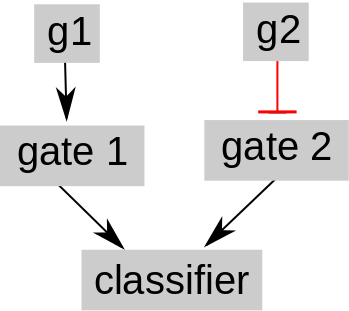
\includegraphics[width=3cm]{constraints_06.png}
 \end{column}
 \begin{column}{0.8\textwidth}
 \begin{tabular}{|c|c|c|c|c|c|c|c|}
  \hline
  ID&	Annots&	g1&	g2&	g3& gate1& gate2& classifier\\
  \hline
  1&	0&	1&	1&	0& 1& 0& healthy\\
  2&	0&	0&	0&	1& 0& 1& healthy\\
  3&	1&	0&	1&	0& 0& 0& healthy\\
  \hline
 \end{tabular}
 \end{column}
 \end{columns}
 \vspace{1.5cm}
 \texttt{
  classifier(TissueID, healthy) :-\\
    \quad not gate\_fires(GateID, TissueID),\\
    \quad is\_gate\_id(GateID), is\_tissue\_id(TissueID).\\
 }
 \vspace{0.3cm}
 \texttt{
  classifier(TissueID, cancer) :-\\
    \quad not classifier(TissueID, healthy),\\
    \quad is\_tissue\_id(TissueID).
 }
\end{frame}

\begin{frame}[fragile]{Consistency of classifier with data}
 \begin{columns}  
 \begin{column}{0.25\textwidth}
 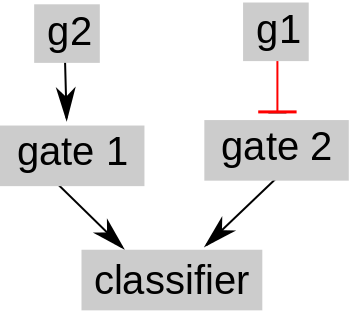
\includegraphics[width=3cm]{constraints_07.png}
 \color{my_example_color}
  \begin{Verbatim}[fontsize=\small]
  gate_input(1,positive,g2).
  gate_input(2,negative,g1).
  \end{Verbatim}
 \end{column}
 \begin{column}{0.8\textwidth}
 \begin{tabular}{|c|c|c|c|c|c|c|c|}
  \hline
  ID&	Annots&	g1&	g2&	g3& gate1& gate2& classifier\\
  \hline
  1&	0&	1&	1&	0& 1& 0& healthy\\
  2&	0&	0&	0&	1& 0& 1& healthy\\
  3&	1&	0&	1&	0& 1& 1& cancer\\
  \hline
 \end{tabular}
 \end{column}
 \end{columns}
 \vspace{1.5cm}
  \begin{verbatim}
  :- tissue(TissueID,healthy), classifier(TissueID,cancer).
  :- tissue(TissueID,cancer),  classifier(TissueID,healthy).
 \end{verbatim}
\end{frame}


\begin{frame}[fragile]{Optimization}
 \begin{itemize}
  \item single objective
  \begin{verbatim}
  #minimize{ 1,GateID:gate_input(GateID,Sign,MiRNA) }.
 \end{verbatim}
  \item with priorities
  \begin{verbatim}
  #minimize{ 1@1,GateID:gate_input(GateID,Sign,MiRNA) }.
  #minimize{ 1@2,MiRNA: gate_input(GateID,Sign,MiRNA) }.
 \end{verbatim}
  \item weighted sum
  \begin{verbatim}
  #minimize{ 1@1,GateID:gate_input(GateID,Sign,MiRNA) }.
  #minimize{ 8@1,MiRNA: gate_input(GateID,Sign,MiRNA) }.
 \end{verbatim}
 \end{itemize}
\end{frame}

\begin{frame}{Priorities matter}
 \begin{center}
 
 \begin{tabular}{|c|c|c|c|c|c|c|c|}
  \hline
  ID&	Annots&	g1&	g2&	g3& g4& g5\\
  \hline
  1&	1&	0&	0&	1& 1& 1\\
  2&	1&	0&	1&	0& 1& 1\\
  3&	1&	0&	1&	1& 1& 1\\
  4&	1&	1&	0&	0& 1& 1\\
  5&	1&	1&	0&	1& 1& 1\\
  6&	1&	1&	1&	0& 1& 1\\
  7&	1&	1&	1&	1& 1& 1\\
  8&	0&	0&	0&	0& 0& 1\\
  9&	0&	0&	0&	0& 1& 0\\
  10&	0&	0&	0&	0& 0& 0\\
  \hline
 \end{tabular}\\\vspace{1cm}
 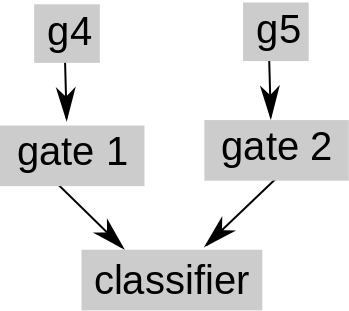
\includegraphics[width=3cm]{optimization_01.png}
 \hspace{1cm}
 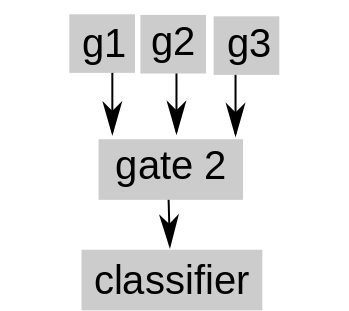
\includegraphics[width=3cm]{optimization_02.png}
 \end{center}
\end{frame}


\begin{frame}{Summary}
 \begin{itemize}
  \item 
  
 \end{itemize}

\end{frame}



\begin{frame}{Remarks}
 \begin{itemize}
  \item mapping \texttt{GateID} to \texttt{GateType}: how to break symmetries?
 \end{itemize}

\end{frame}

\end{document}

 